\section{Preliminary Results}
While our NLP analysis remains in progress, our causal findings suggest substantial changes in Stack Overflow usage patterns. Beyond the volume reduction, we observed a fundamental shift in the correlation structure between Stack Exchange forums after ChatGPT's release, as visualized in Figure \ref{fig:app-correlation_matrix} in the \appref{app:did}.\\

This dramatic weakening of correlations (from 0.76-0.87 to 0.18-0.65) suggests that ChatGPT has reduced question volume and potentially altered the relationship between programming questions and those in other knowledge domains. This finding motivates our hypothesis that the content and nature of Stack Overflow questions have fundamentally changed in the post-ChatGPT era -- a hypothesis we further strengthened by the following results of complexity scores and term frequencies.

%%%%%%%%%%%%%%%%%%%%%%%%%%%%%%%%%%%%%%%%%%%%%%%%%%%%%%%%%%%%%%%%%%%%%%%%%%%%%%%%%%%%%%%%%%%%%%%%

\subsection{Question Complexity Impact}

The average treatment effect on the treated (ATT) indicates a significant increase in our standardized complexity measure of 0.059 standard deviations (cf. \tableref{tab:csscore_did_results}), as shown in Figure \ref{fig:cscore_synthetic_control}. This effect remains robust when including time-fixed effects and various covariates (ATT = 0.073, SE = 0.010).  

\begin{figure}[H]
    \centering
    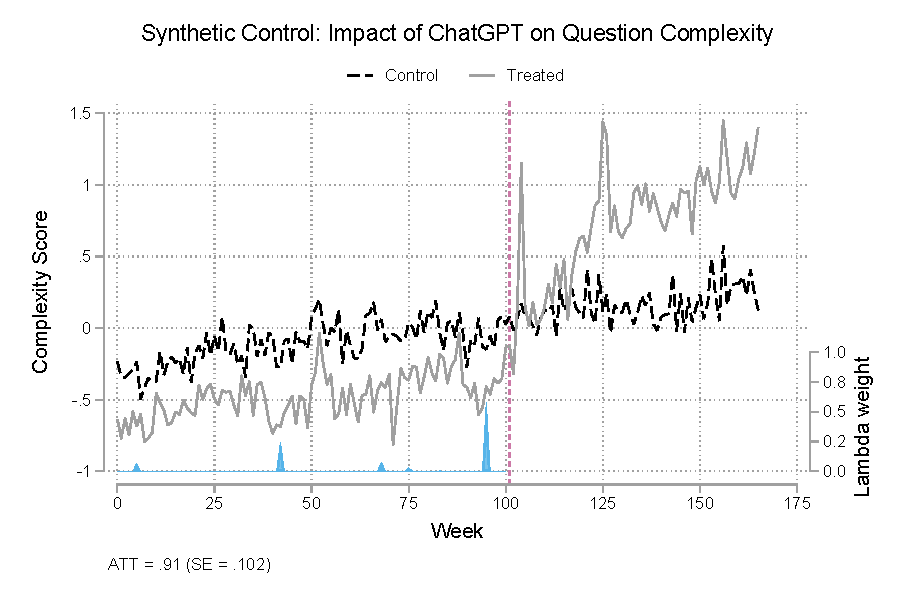
\includegraphics[width=1\linewidth]{imgs/stata/sdid_nlp_trends101.pdf}
    \caption{Synthetic DiD: Question complexity}
    \label{fig:cscore_synthetic_control}
\end{figure}

\begin{table}[H]
    \centering
    \caption{Impact of ChatGPT on Stack Overflow Question Complexity}
    \label{tab:csscore_did_results}
    \begin{tabular}{lccc}
    \toprule
    & \multicolumn{3}{c}{Dependent variable: Complexity Score} \\
    \cmidrule(lr){2-4}
    & (1) & (2) & (3) \\
    \midrule
    Treatment Effect         & 0.084$^{***}$ & 0.059$^{***}$ & 0.073$^{***}$ \\
    & (0.011)       & (0.014)       & (0.010) \\
    &               &               & \\
    \midrule
    Model                    & Basic DiD     & Synthetic DiD & Synthetic DiD \\
    Time fixed effects       & Yes           & Yes           & Yes \\
    Group fixed effects      & Yes           & Yes           & Yes \\
    Month covariates         & No            & No            & Yes \\
    \midrule
    Observations             & 1,328         & 1,328         & 1,328 \\
    Number of groups         & 8             & 8             & 8 \\
    Pre-treatment periods    & 101           & 101           & 101 \\
    Post-treatment periods   & 65            & 65            & 65 \\
    \bottomrule
    \multicolumn{4}{p{1\linewidth}}{\footnotesize \textit{Notes:} Standard errors in parentheses, clustered at the group level. $^{*}$ p$<$0.1, $^{**}$ p$<$0.05, $^{***}$ p$<$0.01. The dependent variable is the standardized complexity score calculated at the individual question level. Each question's complexity is measured as the average of four z-standardized components: tag count, code length, body length, and title length. Treatment is defined as the period after ChatGPT's release (November 30, 2022). Models 1-2 use traditional DiD specifications, while Model 3 uses synthetic control methods with month covariates.} \\
    \end{tabular}
\end{table}

Our complexity scores (cf. \equationref{eq:cscore}), capture multiple dimensions of question sophistication, providing a comprehensive measure of question complexity at the individual level. The traditional DiD regression also confirms this effect (cf. \tableref{tab:csscore_event_study}), with consistent findings across various model specifications. Figure \ref{fig:cscore_event_study} presents the event study results, demonstrating both the immediate impact following ChatGPT's introduction and the persistence of this effect throughout the post-treatment period. 

\begin{figure}[H]
    \centering
    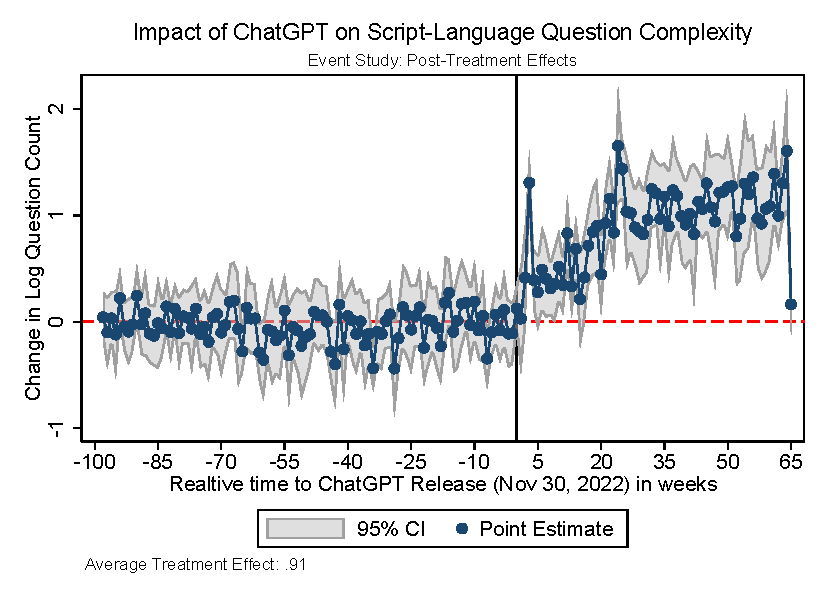
\includegraphics[width=1\linewidth]{imgs/stata/event_study_nlp.pdf}
    \caption{Event study complexity score development}
    \label{fig:cscore_event_study}
\end{figure}

\begin{table}[H]
    \centering
    \caption{Event Study: Post-Treatment Effects Over Time}
    \label{tab:csscore_event_study}
    \begin{tabular}{lccc}
    \toprule
    Time Period & Estimate & SE & 95\% CI \\
    \midrule
    Week 1-4 after treatment   & 0.016 & 0.025 & [-0.033, 0.065] \\
    Week 5-12 after treatment  & 0.028 & 0.022 & [-0.015, 0.071] \\
    Week 13-24 after treatment & 0.064 & 0.018 & [0.029, 0.099] \\
    Week 25-36 after treatment & 0.078 & 0.015 & [0.049, 0.107] \\
    Week 37-48 after treatment & 0.083 & 0.017 & [0.050, 0.116] \\
    Week 49-60 after treatment & 0.081 & 0.019 & [0.044, 0.118] \\
    Week 61-65 after treatment & 0.092 & 0.020 & [0.053, 0.131] \\
    \midrule
    Overall treatment effect & 0.059 & 0.014 & [0.032, 0.086] \\
    \bottomrule
    \multicolumn{4}{p{0.85\linewidth}}{\footnotesize \textit{Notes:} Results from synthetic DiD event study analysis. Estimates show the change in complexity score for Stack Overflow questions relative to the synthetic control group across different post-treatment time periods. Weeks 13-65 effects are statistically significant at the 5\% level, while the initial 1-12 week periods show positive but statistically insignificant effects.} \\
    \end{tabular}
\end{table}

The event study in Figure \ref{fig:cscore_event_study} reveals that while there was an initial positive but non-significant effect in the first twelve weeks after ChatGPT's release, this effect became statistically significant and stronger from week 13 onward. The impact has persisted and strengthened over time, with the largest effect observed in the most recent period (weeks 61-65), suggesting a fundamental shift in how developers utilize Stack Overflow rather than a temporary adjustment.

%%%%%%%%%%%%%%%%%%%%%%%%%%%%%%%%%%%%%%%%%%%%%%%%%%%%%%%%%%%%%%%%%%%%%%%%%%%%%%%%%%%%%%%%%%%%%%%

\subsection{Analysis of Question Content Changes}

The TF-IDF analysis reveals patterns consistent with our complexity findings (cf.~\figureref{fig:tfidf}). Terms related to troubleshooting and debugging (e.g., \enquote{error}, \enquote{issue}, \enquote{expect}), as well as technical infrastructure terms (\enquote{version}, \enquote{package}, \enquote{library}) showed significant increases in importance, while terms associated with basic programming concepts (\enquote{array}, \enquote{loop}, \enquote{list}) decreased significantly. These shifts in term importance indicate that ChatGPT has likely absorbed simpler programming questions, leaving Stack Overflow to serve more complex, specific troubleshooting needs.\\

Notably, conversational terms (\enquote{like}, \enquote{want}, etc.) also decreased in importance, suggesting a shift toward more technical, problem-specific language in post-ChatGPT questions. This aligns with our hypothesis that questions remaining on Stack Overflow have become more specialized and technical in nature.

\begin{figure}[H]
    \centering
    \includesvg[width=1\linewidth]{imgs/term_significance_plot.svg}
    \caption{Top 10 increases and decreases in TF-IDF scores after ChatGPT's introduction}
    \label{fig:tfidf}
\end{figure}

The linguistic changes revealed through our TF-IDF analysis provide qualitative context for the quantitative complexity increases observed in our Synthetic DiD model. The notable shift toward troubleshooting terminology coupled with decreased prevalence of basic programming terms suggests that ChatGPT has fundamentally altered the nature of questions on Stack Overflow, not just their volume or overall complexity.

%%%%%%%%%%%%%%%%%%%%%%%%%%%%%%%%%%%%%%%%%%%%%%%%%%%%%%%%%%%%%%%%%%%%%%%%%%%%%%%%%%%%%%%%%%%%%%%

\subsection{Interpretation}

These findings support our hypothesis that ChatGPT has altered information-seeking behavior in programming communities. Developers now appear to reserve simpler questions for ChatGPT while turning to Stack Overflow for more complex programming challenges that require human expertise. The magnitude of this effect—approximately 0.059 standard deviations increase in question complexity—represents a modest but statistically significant shift in the types of questions users bring to Stack Overflow.\\

To put this effect size in context, it represents a meaningful change in question complexity, particularly given that the complexity measure was calculated at the individual question level using standardized metrics across all questions in our dataset. The gradual increase in effect size over time further suggests that this is not merely a temporary adjustment but rather reflects an evolving shift in how programmers allocate their questions between AI tools and human-moderated forums.\\

This empirical evidence points to a complementary relationship between AI-powered assistants and human-moderated Q\&A forums, with each platform serving distinct informational needs within the programming community. Stack Overflow appears to be evolving toward a repository for more complex programming questions, while more straightforward queries may be increasingly handled through interaction with large language models like ChatGPT.